% !TEX TS-program = xelatex
\documentclass[9pt, aspectratio=169]{beamer}

% \usepackage{lmodern}
\usepackage{amsmath}
\usepackage{amssymb}
\usepackage{physics}
\usepackage{bm}
\usepackage{graphicx}
\usepackage{tikz}
\usepackage{pgfplots}
\usepackage{multirow}
\pgfplotsset{compat=1.18}

\usetheme{metropolis}
\usepackage{fontspec}
\usepackage{anyfontsize}
\usepackage[sfdefault]{FiraSans}
\usepackage[scaled=1.15]{newtxmath}

\definecolor{Foreground}{RGB}{22, 22, 22}
\definecolor{Background}{RGB}{244, 244, 244}
\definecolor{Blue100}{RGB}{0, 17, 65}
\definecolor{Blue90}{RGB}{0, 29, 108}
\definecolor{Blue80}{RGB}{0, 45, 156}
\definecolor{Blue70}{RGB}{0, 67, 206}
\definecolor{Blue60}{RGB}{15, 95, 254}
\definecolor{Blue50}{RGB}{69, 137, 255}
\definecolor{Blue40}{RGB}{120, 169, 255}
\definecolor{Blue30}{RGB}{166, 200, 255}
\definecolor{Blue20}{RGB}{208, 226, 255}
\definecolor{Blue10}{RGB}{237, 245, 255}
\definecolor{Red}{RGB}{218, 30, 40}
\definecolor{Orange}{RGB}{255, 131, 43}
\definecolor{Yellow}{RGB}{253, 220, 105}
\definecolor{Green}{RGB}{25, 128, 56}
\definecolor{Grey05}{RGB}{240, 240, 240}
\definecolor{Grey10}{RGB}{224, 224, 224}
\definecolor{Grey15}{RGB}{211, 211, 211}
\definecolor{Grey20}{RGB}{198, 198, 198}
\definecolor{Grey30}{RGB}{168, 168, 168}
\definecolor{Grey40}{RGB}{141, 141, 141}
\definecolor{Grey50}{RGB}{111, 111, 111}
\definecolor{Grey60}{RGB}{82, 82, 82}
\definecolor{Grey70}{RGB}{57, 57, 57}
\definecolor{Grey80}{RGB}{38, 38, 38}
\definecolor{Grey90}{RGB}{22, 22, 22}
\definecolor{White}{RGB}{255, 255, 255}
\definecolor{Black}{RGB}{0, 0, 0}



\usetikzlibrary{patterns, positioning, arrows.meta, math}
\tikzset{
    nota/.style={align=center, fill=Grey10, inner sep=0.5cm, font=\normalsize},
    titolo nota/.style={align=center, color=Blue50, font=\normalsize},
    etichetta/.style = {fill=white, fill opacity=0.9, text opacity=1, text=black, rounded corners, inner sep=2pt},
    freccia/.style = {arrows = {-Stealth}}
}

\title{\texorpdfstring{\addfontfeature{LetterSpace=3.0}}{} QUANTUM FISHER INFORMATION AS A TOOL FOR DETECTING \\ TOPOLOGICAL PHASES}
\author{\textbf{Sunny Pradhan}, Federico Dell'Anna, Elisa Ercolessi}
\institute{QUANTUM Group @ University of Bologna, Italy\\INFN, Sezione di Bologna, Italy}
\date{}
\titlegraphic{
    \begin{tikzpicture}[overlay, remember picture]
        \node[above=1.5cm, anchor=center] at (current page.250) {
\includegraphics[width=2.25cm]{figures/unibo.pdf}};
        \node[above=1.5cm, anchor=center] at (current page.290) {
\includegraphics[width=1.75cm]{figures/infn_logo.pdf}};
    \end{tikzpicture}
}


\begin{document}
\maketitle

\begin{frame}
    \begin{columns}
        \column[t]{0.5\textwidth}
        \textbf{Multipartite entanglement}
        \begin{itemize}
            \item $n$-separability
                \begin{equation*}
                    \ket{\psi} = \underbrace{\ket{\phi_1} \otimes \cdots \otimes \ket{\phi_n} }_{\text{factorizes in $n$ terms}}
                \end{equation*}
            \item \textbf{$k$-party entanglement}
                \begin{equation*}
                    % \ket{\psi} = \ket{\phi_1} \otimes \ket{\phi_2} \otimes \cdots \otimes \ket{\phi_m},
                    \ket{\psi} =  \bigotimes_{i} \ket{\phi_i}, \quad \text{ $\ket{\phi_i}$ involves at most $k$ parts}
                \end{equation*}
        \end{itemize}

        \column[t]{0.5\textwidth}
        \textbf{Quantum Fisher Information}

        limit to the achievable precision in a phase estimation protocol $\rho \to \rho(\theta)$
        \begin{equation*}
            (\Delta \theta)^2 \geq
            \frac{1}{m F} \geq
            \frac{1}{m F_Q}
        \end{equation*}
        \begin{itemize}\small
            \item $F$: Fisher information
            \item $F_Q$: quantum Fisher information
            \item $f_Q = F_Q / L$: QFI density
        \end{itemize}
    \end{columns}

    \vspace*{0.3cm}
    \hrule
    \vspace*{0.3cm}


    \begin{columns}
        \column{0.45\textwidth}
        \centering
        \textbf{Entanglement criterion}

        \vspace*{0.1cm}

        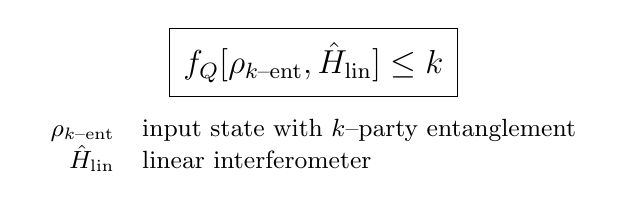
\begin{tikzpicture}
            \node[draw=black, inner sep=5pt, font=\large] (crit) at (0,0) {
                $f_Q[\rho_{k \text{--ent}}, \hat{H}_{\text{lin}}] \leq k$
            };
            \node[below=0.1cm of crit, font=\small] {
                $
                \begin{array}{rl}
                    \rho_{k \text{--ent}} & \text{input state with $k$--party entanglement} \\
                    \hat{H}_{\text{lin}} & \text{linear interferometer}
                \end{array}
                $
            };
        \end{tikzpicture}

        \column{0.45\textwidth}
        We look at the multipartite entanglement structure of symmetry protected topological phases using quantum Fisher information of non-local operators

    \end{columns}

\end{frame}

\begin{frame}{Long-range Kitaev chain}
    one-dimensional $p$-wave superconductor with \textbf{long-range coupling} $\sim 1/r^{\alpha}$

    \small
    \begin{equation*}
        H = \sum_{j} \qty[
            -t c_j^{\dagger} c_{j+1}
            -\mu \qty( c_j^{\dagger} c_j - \frac{1}{2} )
            + \frac{\Delta}{2} \sum_{r} \boxed{\frac{1}{r^{\alpha}} c_j^{\dagger} c_{j+r}}
            + \text{h.c.}
        ]
    \end{equation*}

    \begin{columns}\small
        \column{0.4\textwidth}
        \textbf{QFI of non-local spin degrees of freedom}
        \begin{itemize}\footnotesize
            \item $\sigma_j^+ = c^{\dagger}_j e^{i \pi \sum_{i < j} c_i^{\dagger} c_i} $, ~~$\sigma_j^- = e^{i \pi \sum_{i < j} c_i^{\dagger} c_i} c_j $
            \item $\hat{H}_{\text{lin}}^{\,\rho} = \sum_{j} \sigma^{\rho}_{j} $, ~$\rho=x,y$
        \end{itemize}
        We look at the scaling of $f_Q[\ket{\text{gs}}, \hat{H}_{\text{lin}}^{\,\rho}]$ with the system size $L$
        \\[10pt]
        \fbox{\parbox{\textwidth}{The scaling can be computed analytically \\ using \textbf{Toeplitz determinants}}}

        \column{0.5\textwidth}
        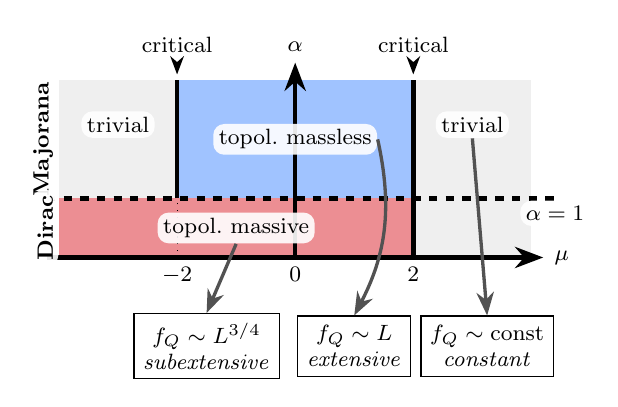
\begin{tikzpicture}[
    scale=0.75,
    font=\footnotesize,
    punto/.style = {circle, inner sep=0pt, minimum size=2pt, fill=black},
    massless/.style = {fill=Blue40, fill opacity=0.7},
    trivial/.style = {fill=Grey10,  fill opacity=0.5},
    massive/.style = {fill=Red,   fill opacity=0.5},
    etichetta spettro/.style = {above=-0.25cm, font=\normalsize, fill=Grey10, fill opacity=0.9, text opacity=1, rounded corners, inner sep=2pt}
    ]

    %%% Phases
    % massless
    \path[massless] (-2,1) rectangle (2,3);
    % massive
    \path[massive]  (-4,1) rectangle (2,0);
    % trivial
    \path[trivial] (-4,1) rectangle (-2,3);
    \path[trivial] (2,0) rectangle (4,3);

    % sector separator
    \draw[dashed, ultra thick] (-4.2,1) -- (4.4,1) node [below, etichetta] {$\alpha = 1$};

    % critical line
    \draw[ultra thick] (2,0) -- (2,3);
    \draw[dotted]     (-2,0) -- (-2,1);
    \draw[ultra thick] (-2,1) -- (-2,3);

    %%% Axis
    \draw[ultra thick, freccia] (0,0) -- (0,3.3) node [above] {$\alpha$};
    \draw[ultra thick, freccia] (-4.2,0) -- (4.2,0) node [right] {$\mu$};
    \draw (2,0) node [below] {$2$};
    \draw (-2,0) node [below] {$-2$};
    \draw (0,0) node [below] {$0$};


    % labels
    \node [etichetta] (massless) at (0,2)  {topol.~massless};
    \node [etichetta] (trivial1) at (-3,2.25) {trivial};
    \node [etichetta] (trivial2) at (3,2.25)  {trivial};
    \node [etichetta] (massive)  at (-1,0.5)  {topol.~massive};

    \draw[Stealth-, thick] (2,3.1) -- (2,3.3) node [above] {critical};
    \draw[Stealth-, thick] (-2,3.1) -- (-2,3.3) node [above] {critical};

    \draw (-4, 2)    node [anchor=south, etichetta, rotate=90] {\textbf{Majorana}};
    \draw (-4, 0.5)  node [anchor=south, etichetta, rotate=90] {\textbf{Dirac}};

    \node[align=center, draw=black] (subext) at (-1.5, -1.5) {$f_Q \sim L^{3/4}$\\ \emph{subextensive}};
    \node[align=center, draw=black] (ext)    at ( 1.0, -1.5) {$f_Q \sim L$\\ \emph{extensive}};
    \node[align=center, draw=black] (const)  at ( 3.25, -1.5) {$f_Q \sim \text{const}$\\ \emph{constant}};

    \draw[very thick] (massive.south)  edge[Grey60, freccia] (subext.north);
    \draw[very thick] (massless.east)  edge[Grey60, freccia, bend left=20] (ext.north);
    \draw[very thick] (trivial2.south) edge[Grey60, freccia] (const.north);
\end{tikzpicture}


    \end{columns}
\end{frame}


\begin{frame}{Bilinear-Biquadratic model}
    most general $SU(2)$--invariant isotropic spin-$1$ Hamiltonian

    \small
    \begin{equation*}
        H = J \sum_{i} \qty[
            \bm{S}_i \cdot \bm{S}_{i+1}
            - \beta \qty( \bm{S}_i \cdot \bm{S}_{i+1} )^2
        ]
        = J^{\prime}  \sum_{i} \qty[
            \cos \theta \bm{S}_i \cdot \bm{S}_{i+1}
            - \sin \theta \qty( \bm{S}_i \cdot \bm{S}_{i+1} )^2
        ]
    \end{equation*}

    \begin{columns}\small
        \column{0.35\textwidth}

        \textbf{QFI of string operators}
        \begin{itemize}\footnotesize
            \item $\widetilde{S}_j^z = \left( e^{i \pi \sum_{i < j}  S^z_i } \right) S_j^z$
            \item $\hat{O} = \sum_{j} \widetilde{S}_j^z $
        \end{itemize}
        We look at the scaling of $f_Q[\ket{\text{gs}}, \hat{O}]$ with the system size $L$


        \column{0.65\textwidth}
        \centering
        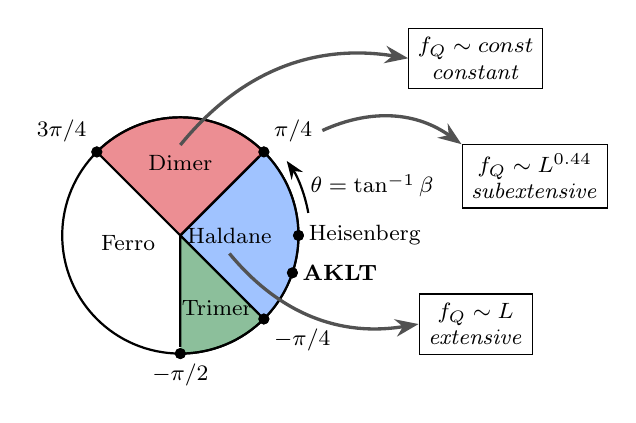
\begin{tikzpicture}[
        % scale=5,
        scale=1.5,
        font=\footnotesize,
        dot/.style = {circle, inner sep=0pt, minimum size=4pt, fill=black},
        thick,
        etichetta grafico/.style = {above=0.1cm, font=\normalsize, fill=Grey10, fill opacity=0.9, text opacity=1, rounded corners, inner sep=2pt},
        nota grafico/.style = {below=0.2cm, font=\small, fill=Grey10, fill opacity=0.9, text opacity=1, rounded corners, inner sep=2pt, align=center},
        sfondo grafico/.style = {fill=white, draw=black, thin, inner sep=2pt}
    ]
    \node (A) at (45:1)  [dot] {};
    \node (C) at (-45:1) [dot] {};
    \node (D) at (-90:1) [dot] {};
    \node (E) at (135:1) [dot] {};
    \node (H) at (0:1)   [dot] {};
    \node (K) at (-18.44:1) [dot] {};
    \node[above right] (critical) at (A) {$\pi/4$};
    \node[below right] at (C) {$-\pi/4$};
    \node[below]       at (D) {$-\pi/2$};
    \node[above left]  at (E) {$3 \pi / 4$};
    \node[right]       at (H) {Heisenberg};
    \node[right]       at (K) {\textbf{AKLT}};

    \draw (0,0) circle [radius=1];

    \draw[fill=Blue40, fill opacity=0.7] (0,0) -- (C) arc (-45:45:1) -- (0,0);
    \draw[fill=Green, fill opacity=0.5] (0,0) -- (D) arc (-90:-45:1) -- (0,0);
    \draw[fill=Red, fill opacity=0.5] (0,0) -- (A) arc (45:135:1) -- (0,0);

    \node at (45:1)  [dot] {};
    \node at (-45:1) [dot] {};
    \node at (-90:1) [dot] {};
    \node at (135:1) [dot] {};
    \node at (0:1)   [dot] {};
    \node at (-18.44:1) [dot] {};

    \path (A) arc (45:135:1) node (dimer) [below=10pt, midway] {Dimer};
    \path (C) arc (-45:45:1) node (Haldane) [left=6pt, midway] {Haldane};
    \path (D) arc (-90:-225:1) node [above right=10pt, midway] {Ferro};
    \path (C) arc (-45:-90:1) node [above=8pt, pos=0.6] {Trimer};

    \draw[freccia] (10:1.1) arc (10:35:1.1) node [midway, right] {$\theta = \tan^{-1} \beta$};

    \node[align=center, draw=black, thin] (const) at (2.5, 1.5) {$f_Q \sim const$ \\ \emph{constant}};
    \node[align=center, draw=black, thin] (subext) at (3, 0.5) {$f_Q \sim L^{0.44}$ \\ \emph{subextensive}};
    \node[align=center, draw=black, thin] (ext) at (2.5, -0.75) {$f_Q \sim L$ \\ \emph{extensive}};

    \draw[very thick] (Haldane.south) edge[Grey60, freccia, bend right] (ext.west);
    \draw[very thick] (critical.east) edge[Grey60, freccia, bend left] (subext.north west);
    \draw[very thick] (dimer.north) edge[Grey60, freccia, bend left] (const.west);

\end{tikzpicture}




    \end{columns}
\end{frame}
\end{document}
